% $> xelatex spsi.tor.presentacion.tex
% o bien
% $> lualatex spsi.tor.presentacion.tex
\documentclass[spanish]{beamer}

\usepackage[es-tabla]{babel}

\usepackage{graphics,tikz}
\usetikzlibrary{automata, positioning, arrows}

\usepackage{pgfplotstable}
\pgfplotsset{compat=1.16}

\usepackage{adjustbox}
\usepackage{booktabs}
\usepackage{multirow}
\usepackage{enumitem}

%%% FUENTES

\usepackage[no-math]{fontspec}
\setmainfont{Libertinus Serif}
\setsansfont{Libertinus Sans}
\setmonofont{Libertinus Mono}

\usepackage[math-style=TeX]{unicode-math}
\setmathfont{Libertinus Math}

\usepackage{pifont}
\newcommand{\cmark}{\ding{51}}%
\newcommand{\xmark}{\ding{55}}%

%%% COLORES

\definecolor{background}{HTML}{F5F5F4}
\definecolor{foreground}{HTML}{3F3F3F}
\definecolor{strings}{HTML}{ED982C}
\definecolor{operators}{HTML}{CF4818}
\definecolor{identifiers}{HTML}{9A71BA}
\definecolor{keywords}{HTML}{5486C8}
%\definecolor{keywords}{HTML}{54BFC7}
\definecolor{numbers}{HTML}{80951D}
\definecolor{comments}{HTML}{AFAFAF}

%%% LISTINGS

\usepackage{listings}

\lstset{
  numbers=left,
  belowcaptionskip=1\baselineskip,
  basicstyle=\scriptsize\ttfamily\color{foreground},
  keywordstyle=\color{keywords},
  commentstyle=\color{comments},
  stringstyle=\color{strings},
  identifierstyle=\color{identifiers},
  numberstyle=\color{foreground},
  xleftmargin=2em,
  framexleftmargin=1.5em,
  breaklines=true,
  showstringspaces=false,
  tabsize=2
}

% Bibliografía

\usepackage[sorting=none, style=apa, isbn=true]{biblatex}
\DefineBibliographyStrings{spanish}{
  urlseen = {Consultado},
  retrieved = {Consultado},
}
\addbibresource{bibliografia.bib}

%%% AJUSTES DE BEAMER

%\usefonttheme{professionalfonts}

\setlength{\leftmargini}{0cm}
\setlength{\leftmarginii}{2em}

\setbeamertemplate{navigation symbols}{}

\setbeamerfont{title}{series=\bfseries}

%\setbeamertemplate{frametitle}{\color{foreground}\vspace*{1cm}\bfseries\insertframetitle\par\vskip-6pt}
\setbeamerfont{frametitle}{series=\bfseries}
\setbeamercolor{frametitle}{fg=foreground}
\setbeamerfont{framesubtitle}{size=\normalfont\small}
\setbeamercolor{framesubtitle}{fg=foreground}

\setbeamercolor{background canvas}{bg=background}

\setbeamercolor{normal text}{fg=foreground}
\setbeamercolor{alerted text}{fg=foreground}
\setbeamercolor{block title}{fg=foreground}
\setbeamercolor{alerted text}{fg=foreground}

\setbeamercolor{itemize item}{fg=foreground}
\setbeamercolor{enumerate item}{fg=foreground}

\setbeamertemplate{itemize items}[circle]
\setitemize{
  label=\usebeamerfont*{itemize item}
  \usebeamercolor[fg]{itemize item}
  \usebeamertemplate{itemize item}
}

\setbeamercolor*{title}{fg=foreground}
\setbeamercolor{qed symbol}{fg=foreground}

\usebeamercolor[fg]{normal text}

\setbeamertemplate{footline}[frame number]
\setbeamerfont{page number in head/foot}{size=\small}

\setbeamercolor{section in toc}{fg=foreground}
\setbeamerfont{section in toc}{series=\bfseries}

\setbeamercolor{caption name}{fg=foreground}
\setbeamerfont{caption name}{series=\bfseries}

\setbeamercolor{bibliography entry note}{fg=foreground}
\setbeamercolor{bibliography entry author}{fg=foreground!40!black}

\hypersetup{
  colorlinks=true,
  citecolor=numbers,
  urlcolor=operators,
  linkcolor=foreground
}

%%% INFORMACIÓN DEL DOCUMENTO

\title{Curvas elípticas en la criptografía}
\subtitle{Historia de las Matemáticas}
\author{
  Sofía Almeida Bruno \texorpdfstring{\\}{}
  Antonio Coín Castro \texorpdfstring{\\}{}
  José María Martín Luque
}
\institute{\normalsize Universidad de Granada}
\date{17 de diciembre de 2019\texorpdfstring{\\}{} \small Curso 2019-2020}

\begin{document}

\maketitle

\begin{frame}{Índice}
  \tableofcontents
\end{frame}

\section{Criptografía}
\begin{frame}{Criptografía}
  \begin{itemize}
    \item Objetivo: transmitir información confidencial a través de un canal inseguro.
    \item Ya en la antigüedad se usaba en contextos bélicos o políticos. Un ejemplo es el \textit{cifrado del César}:
    \[x \mapsto x + 3 \mod 26.\]
    \item En la \textit{era de la información} experimenta una evolución sin precedentes.
    \item Los sistemas actuales basan su seguridad en problemas matemáticos \textit{difíciles} de resolver.
  \end{itemize}
\end{frame}

% Comentar el origen del nombre
\section{Curvas elípticas}
\begin{frame}{Curvas elípticas}{Definición (I)}
  \begin{itemize}
    \item Una \textit{curva elíptica} sobre un cuerpo $K$ es una curva proyectiva no singular $E \subset \mathbb{P}^2(K)$ definida por una ecuación de la forma
    \[ y^2 + a_1xy + a_3y = x^3 +a_2x^2 + a_4x + a_6,\]
    con cada \(a_i \in K\).
    \item Si la característica de \(K\) es distinta de \(2\) y \(3\) podemos simplificar la ecuación, obteniendo la \textit{ecuación de Weierstrass}
    \[y^2 = x^3 + Ax + B,\]
    con \(A, B \in K\).
  \end{itemize}

\end{frame}

\begin{frame}{Curvas elípticas}{Definición (II)}
  Se puede comprobar que la curva corta a la recta del infinito en un único punto.
  \[ E = E(K) = \left\{ (x, y) \in K \times K : y^2 = x^3 + Ax + B\right\} \cup \big\{\mathcal{O}\big\}.\]
  \begin{itemize}
    \item \(\mathcal O\) es el punto del infinito con coordenadas homogéneas \([0:1:0]\).
    \item La condición de no singularidad se traduce en \(4A^3 + 27B^2 \neq 0\).
  \end{itemize}

\end{frame}

\begin{frame}[fragile]{Curvas elípticas}{Ejemplos (I)}
  \begin{figure}[h]
    \centering
    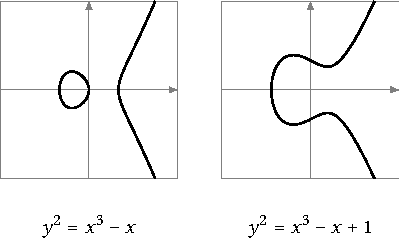
\includegraphics[width=.75\textwidth]{img/ejemplos-curvas}
    \caption{Ejemplos de curvas elípticas sobre $\mathbb{R}$. Basado en \parencite{eichlseder_elliptic_2016}.}
    \label{fig:curvas}
  \end{figure}
\end{frame}

% Decir que las curvas sobre cuerpos finitos son las que se usan en criptografía, pero son más difíciles de visualizar. Todo es mod p.
\begin{frame}[fragile]{Curvas elípticas}{Ejemplos (II)}
  \begin{figure}[h]
    \centering
    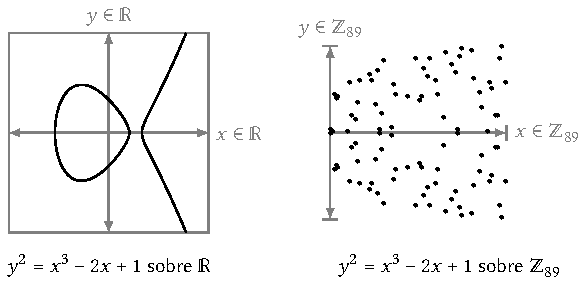
\includegraphics[width=.85\textwidth]{img/cuerpos-curvas}
    \caption{Ejemplo de una curva elíptica sobre $\mathbb{R}$ y sobre $\mathbb{Z}_{89}$. Basado en \parencite{eichlseder_elliptic_2016}.}
    \label{fig:curvas-finitos}
  \end{figure}
\end{frame}

\begin{frame}{Suma de puntos}
  % Hablar de:
  % - método algebraico (lo que vamos a contar se hace con ecuaciones)
  % - las rectas verticales cortan a la curva al menos en el punto del infinito
  \begin{itemize}
    \item Podemos definir una operación suma sobre los puntos de una curva elíptica para obtener un grupo abeliano.
    \item El elemento neutro será el punto \(\mathcal{O}\).
    \item Para visualizar el método, suponemos que el cuerpo base es $\mathbb{R}$.
  \end{itemize}
\end{frame}

\begin{frame}{Suma de puntos}{Elemento neutro}
  \begin{figure}[h]
    \centering
    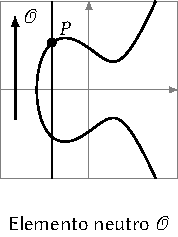
\includegraphics[width=0.35\textwidth]{img/neutro-curvas}
    \caption{Suma del punto del infinito \(\mathcal O\) a un punto en curvas elípticas. Basado en  \parencite{eichlseder_elliptic_2016}.}
    \label{fig:duplicar-curvas}
  \end{figure}
\end{frame}

\begin{frame}{Suma de puntos}{Caso general}
  \begin{figure}[h]
    \centering
    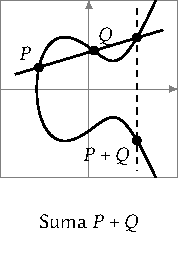
\includegraphics[width=0.35\textwidth]{img/suma-curvas}
    \caption{Suma de puntos en curvas elípticas. Basado en  \parencite{eichlseder_elliptic_2016}.}
    \label{fig:suma-curvas}
  \end{figure}
\end{frame}

\begin{frame}{Suma de puntos}{Elemento inverso}
  \begin{figure}[h]
    \centering
    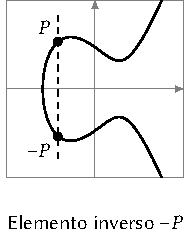
\includegraphics[width=0.35\textwidth]{img/inverso-curvas}
    \caption{Elemento inverso de un punto en curvas elípticas. Basado en  \parencite{eichlseder_elliptic_2016}.}
    \label{fig:inverso-curvas}
  \end{figure}
\end{frame}

\begin{frame}{Suma de puntos}{Duplicar puntos}
  \begin{figure}[h]
    \centering
    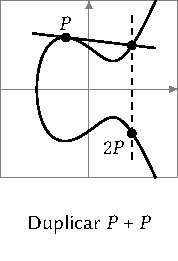
\includegraphics[width=0.35\textwidth]{img/duplicar-curvas}
    \caption{Duplicación de un punto en curvas elípticas. Basado en  \parencite{eichlseder_elliptic_2016}.}
    \label{fig:duplicar-curvas}
  \end{figure}
\end{frame}

\begin{frame}[fragile]{Evolución de las curvas elípticas en la criptografía}{Años 70 - Interés creciente en la criptografía}
  \begin{itemize}
    \item En 1973 la NBS organizó un concurso público para el diseño de un algoritmo de cifrado que el Gobierno pudiera adoptar como estándar.
    \item En 1975 un grupo de investigación de IBM publicó el primer borrador del DES.
    \item La NSA aporta modificaciones y en 1976 la NBS lo aprobó y publicó. %contar que esto generó sospechas etc
    \item Este algoritmo fue reemplazado por AES en 2002.
  \end{itemize}
\end{frame}

\begin{frame}[fragile]{Evolución de las curvas elípticas en la criptografía}{Años 70 - Criptografía de clave pública}
  \begin{itemize}
  \item En 1976 se publicó el artículo \textit{New Directions in Cryptography} donde W. Diffie y M. Hellman proponen por primera vez la idea de cifrado de clave pública. % Explicar en una frase cifrado de clave pública y comentar que hasta el momento la seguridad de los algoritmos dependía solo de que solo los interesados conocieran la clave
  \item Surge el protocolo de intercambio de claves de Diffie y Hellman, que basa su seguridad en la dificultad de resolver el \textit{problema del logaritmo discreto}:

  \begin{quote}
    \vspace{1em}
    Sea \(G\) un grupo y $g \in G$. Dado \(a \in \langle g \rangle\), encuentra \(x\) tal que \(g^x = a\). % Se usa en criptografía con G = grupo multiplicativo de F_p, p primo.
\end{quote}
  \end{itemize}
\end{frame}

\begin{frame}[fragile]{Evolución de las curvas elípticas en la criptografía}{Años 80 - Aparición de las curvas elípticas}
  \begin{itemize}
    \item En 1984 H. Lenstra propone el primer algoritmo que utiliza las curvas elípticas, era un algoritmo de factorización.
    \item En 1985 N. Koblitz y V. Miller proponen un criptosistema basado en el \textit{problema del logaritmo discreto en curvas elípticas}:

    \begin{quote}
      \vspace{.5em}
      Sea $E(\mathbb{F}_p)$ verificando $y^2 =x^3 + Ax + B$. Consideramos $\langle G \rangle$ un subgrupo cíclico de orden $n$ de los puntos de $E$. Dados $P,Q \in \langle G \rangle$ encuentra $x \bmod{n}$ tal que $Q=xP$.
      \vspace{.5em}
      \end{quote}
    \item Protocolo ECDH.
  \end{itemize}
\end{frame}

\begin{frame}[fragile]{Evolución de las curvas elípticas en la criptografía}{Años 80 - Adaptaciones de algoritmos conocidos (I)}
  \begin{itemize}
    \item No parecía que se pudiese adaptar el algoritmo de \textit{index calculus} para computar logaritmos discretos en curvas elípticas.
    \item Había ciertas curvas donde los cálculos eran especialmente eficientes.
    \item Se comienzan a adaptar los algoritmos criptográficos existentes a los grupos de curvas elípticas:
    \begin{itemize}
	    \item ElGamal (1987). % Cifrado de clave pública - Koblitz
	    \item ECDSA (1992).   % Firma
    \end{itemize}
    \item Proporcionaban una seguridad similar con claves de menor tamaño.
  \end{itemize}
\end{frame}

\begin{frame}[fragile]{Evolución de las curvas elípticas en la criptografía}{Años 80 - Adaptación de algoritmos conocidos (II)}
  \begin{itemize}
    \item Se adaptan también algoritmos para resolver el problema del logaritmo discreto en curvas elípticas: % Aclarar que si se consiguiera el cifrado que lo usa no serviría
      \begin{itemize}
	    \item Algoritmo de Pohlig y Hellman.
        \item Algoritmo \textit{baby-step/giant-step} de Shanks, algoritmo \textit{rho} de Pollard. % Tiempo raíz de n
    \end{itemize}

    \item Ataque por emparejamiento de Weil. % SI se dice lo de las curvas supersingulares decir que este algoritmo es especialmente efectivo en ellas
  \end{itemize}

  % Durante los años siguientes a la aparición de la criptografía de la curva elíptica la actitud general de los criptógrafos fue de aceptación y curiosidad, nadie la consideró una amenaza comercial.
  % A finales de los años 80, un grupo amplio de matemáticos empezó a trabajar en el tema ...
\end{frame}

\begin{frame}[fragile]{Evolución de las curvas elípticas en la criptografía}{Años 90 - Enfrentamiento con RSA - Apoyo de la NSA (I)}
  \begin{itemize}
    \item RSA es un criptosistema de clave pública que surgió en 1977 y cuya seguridad radica en el problema de factorización. % éxito comercial, buena aceptación
    \item Los partidarios de la ECC comienzan a luchar por su inclusión en los estándares criptográficos. % (ECDSA no fue incluido hasta 1999 y 2000).
    \item El NIST propone un protocolo de firma desarrollado por la NSA donde la seguridad se basaba en el problema del logaritmo discreto.%  A principios de los 90. Aunque este algoritmo no estaba basado en curvas elípticas, mostró el descontento con RSA que existía por parte de la NSA.
    \end{itemize}
    \end{frame}
\begin{frame}[fragile]{Evolución de las curvas elípticas en la criptografía}{Años 90 - Enfrentamiento con RSA - Apoyo de la NSA (II)}

	La criba general del cuerpo de números provocaba que RSA tuviera que usar claves cada vez más largas. % algoritmo clásico de factorización. Descontento de la NSA. Capacidad de cómputo iba en aumento

\begin{table}[h]
  \centering
  \sffamily
  \begin{tabular}{lccc}
    \toprule
     & \multicolumn{3}{c}{Tamaño en bits} \\
    Periodo & nivel de seguridad & RSA & ECC \\
    \midrule
    Pasado & 80 & 1024 & 160\\
    \multirow[t]{4}{*}{2016-2030} & 112 & 2048 & 224\\
     & 128 & 3072 & 256\\
     & 192 & 7680 & 384\\
     & 256 & 15360 & 512\\
    \bottomrule
  \end{tabular}
  \caption{Recomendaciones del NIST para el tamaño de las claves de RSA y ECC \parencite{barker_recommendation_2016}.}
  \label{tab:rsa-ecc-nist}
\end{table} %Arreglar
\end{frame}

\begin{frame}[fragile]{Evolución de las curvas elípticas en la criptografía}{Años 90 - Enfrentamiento con RSA - Apoyo de la NSA (III)}
    \begin{itemize}
    \item En 1997 RSA Data Security puso una sección en su página web advirtiendo del riesgo que suponía usar la criptografía basada en curvas elípticas.
    \begin{itemize}
        \item Pocos criptógrafos comprendían realmente las curvas elípticas.
	    \item El problema de factorización se había estudiado durante cientos de años.
\end{itemize}
    \item Ese mismo año un miembro de la NSA publica
    el primer artículo en un congreso sobre criptografía que trataba sobre la ECC.
  \end{itemize}
\end{frame}

 \begin{frame}[fragile]{Evolución de las curvas elípticas en la criptografía}{Siglo XXI - Estandarización de la ECC}
    \begin{itemize}
    \item La NSA autorizó en 2003 26 patentes relacionadas
con ECC y en 2005 publicó un artículo en su web donde fomentaba su uso.
    \item RSA eliminó de su web la sección donde criticaba la ECC.
    \item En 2001 surgen algoritmos basados en emparejamientos sobre curvas elípticas: % Emparejamiento: aplicación que parte del producto cartesiano de un subconjunto de la curva
    \begin{itemize}
	    \item Criptosistemas basados en identidad.
	    \item Algoritmos de firma que aprovechan las propiedades de las curvas elípticas.
    \end{itemize}
  \end{itemize}
\end{frame}

\begin{frame}[fragile]{Futuro de las curvas elípticas}
  \begin{itemize}
    \item El poder de computación de los ordenadores cuánticos podría suponer el fin de la criptografía tal y como la conocemos. % Algoritmo de Shor: factorización de enteros. Se puede aplicar para resolver el logaritmo discreto.
    \item El NIST comenzó en 2017 una recogida de propuestas para el desarrollo de nuevos criptosistemas \parencite{computer_security_division_call_2017}. % Se busca que estos basen su seguridad en problemas matemáticos difíciles, distintos del logaritmo discreto y la factorización.
    \item El algoritmo de SIDH se basa en encontrar la relación entre dos curvas elípticas dentro de una gran familia de ellas.
    \end{itemize}
\end{frame}


\begin{frame}[t,allowframebreaks]{Referencias}
  \printbibliography[heading=none]
\end{frame}

\end{document}
